\documentclass[11pt,a4paper]{article}
\usepackage[utf8]{inputenc}
\usepackage[margin=0.8in]{geometry}
\usepackage{graphicx}
\usepackage{hyperref}
\usepackage{booktabs}
\usepackage{tabularx}
\usepackage{enumitem}
\usepackage{xcolor}

% Hyperlink styling
\hypersetup{
    colorlinks=true,
    linkcolor=black,
    urlcolor=blue!75!black,
    citecolor=black
}

\setlength{\parindent}{0pt}
\setlength{\parskip}{5pt}

\begin{document}

% ------------------- Title Header -------------------
\begin{center}
    {\LARGE \textbf{End-to-End CI/CD Pipeline for a Calculator REST API}}\\[0.35em]
    {\large CSE 816 -- Software Production Engineering \quad$|$\quad Mini-Project Report}\\[0.3em]
    {\large \textbf{P. Venkata Rami Reddy} \quad$|$\quad \textbf{[Roll Number: IMTXXXXXXXX]}}
\end{center}
\vspace{-0.5em}
\hrule
\vspace{1em}

% ------------------- Section 1: Overview -------------------
\section{Overview}
A Spring Boot (Java 17, Maven) calculator service exposes \texttt{/api/v1/add}, \texttt{subtract}, \texttt{multiply}, \texttt{divide} and the Actuator health endpoint \texttt{/actuator/health}. Invalid or missing parameters and division by zero return HTTP 400 with a structured JSON error.

\begin{itemize}[leftmargin=*,itemsep=2pt,topsep=2pt]
    \item \textbf{GitHub Repository:} \url{https://github.com/Venkat96r/calculator-devops}
    \item \textbf{Docker Hub Repository:} \url{https://hub.docker.com/r/venkat96r/calculator-api}
    \item \textbf{Tools in Scope:} Git/GitHub, Jenkins (declarative pipeline), Docker (multi-stage image), Docker Compose with Nginx.
\end{itemize}

% ------------------- Section 2: Pipeline Architecture -------------------
\section{Pipeline Architecture}

\begin{figure}[htbp]
    \centering
    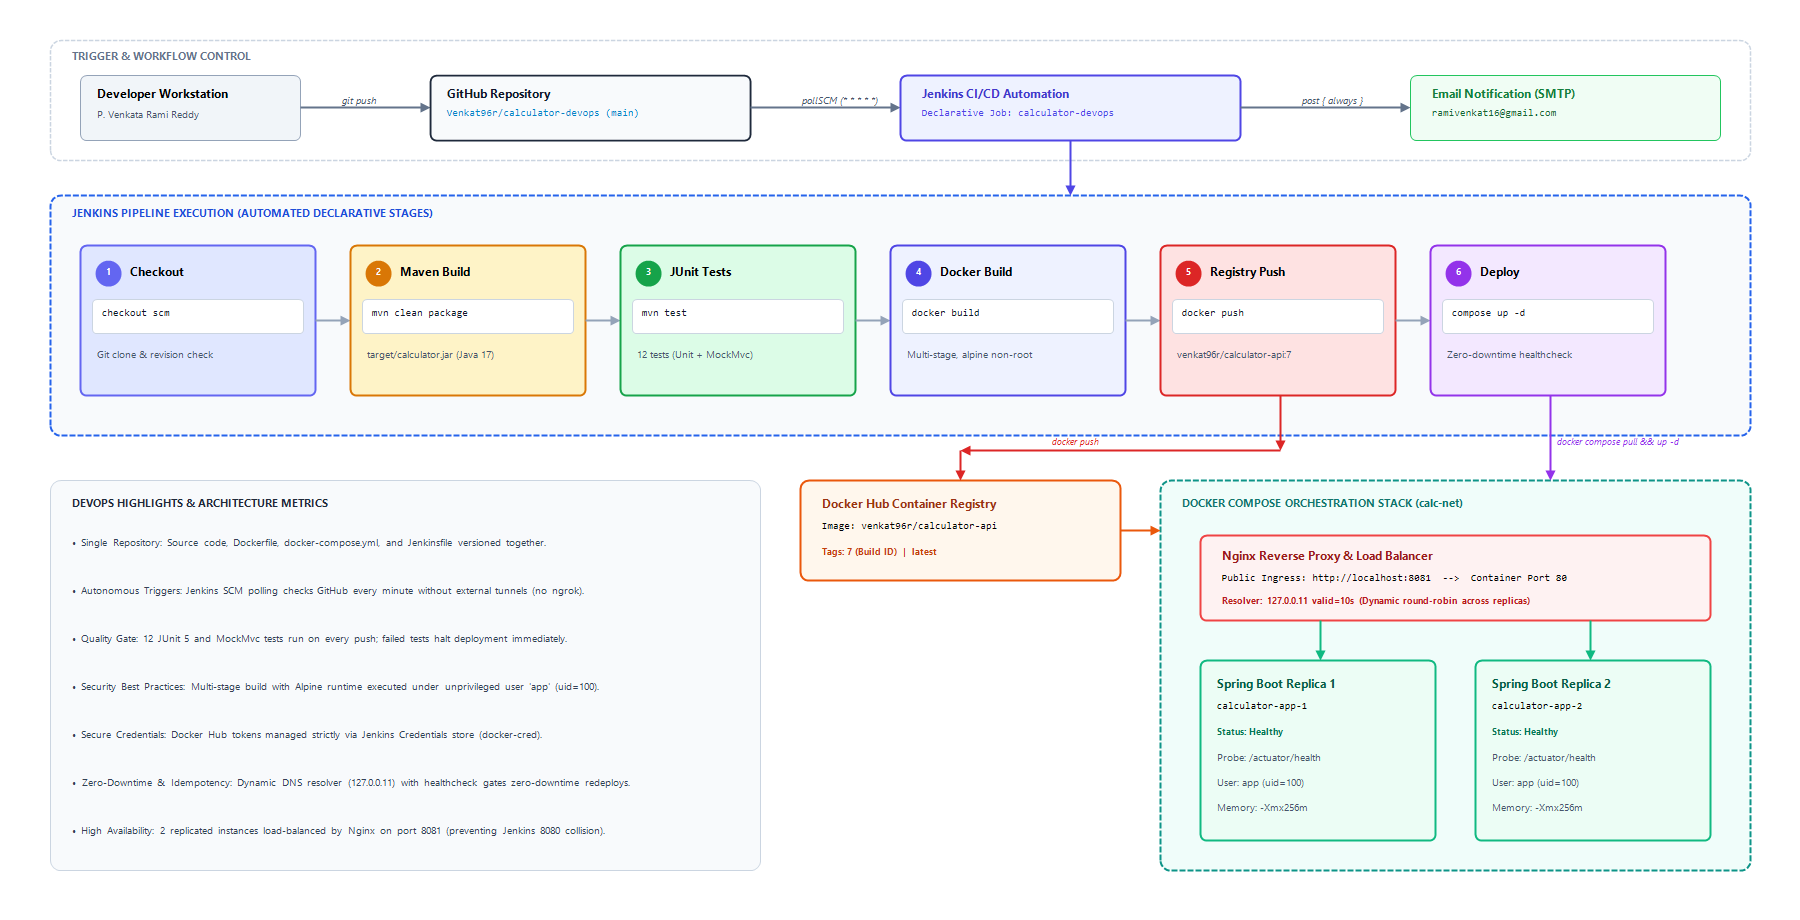
\includegraphics[width=\textwidth]{screenshots/architecture_pipeline.png}
    \caption{End-to-End Pipeline Architecture. A push to \texttt{main} triggers SCM polling; Jenkins executes the six declarative stages and emails the result; the container image is published to Docker Hub and deployed to the two-replica Compose stack fronted by Nginx.}
    \label{fig:arch}
\end{figure}

\vspace{-0.5em}

% ------------------- Section 3: Pipeline Stages -------------------
\section{Pipeline Stages}

\begin{table}[htbp]
\centering
\small
\begin{tabularx}{\textwidth}{l X}
\toprule
\textbf{Stage} & \textbf{Description} \\
\midrule
\textbf{Checkout} & \texttt{checkout scm} pulls the latest commit. The build is triggered automatically by SCM polling (\texttt{pollSCM('* * * * *')}). \\
\addlinespace[2pt]
\textbf{Build} & \texttt{mvn -B clean package -DskipTests} compiles the Java 17 code and packages the executable JAR \texttt{target/calculator.jar}. \\
\addlinespace[2pt]
\textbf{Test} & \texttt{mvn -B test} runs the 5 JUnit 5 unit tests and 7 MockMvc integration tests. The \texttt{junit} step records test results from \texttt{target/surefire-reports/*.xml}; any failure stops the pipeline. \\
\addlinespace[2pt]
\textbf{Docker Build} & Builds the multi-stage image (Stage 1: \texttt{maven:3.9-eclipse-temurin-17} builder with dependency offline cache; Stage 2: slim \texttt{eclipse-temurin:17-jre-alpine} runtime, non-root user \texttt{app:100}, \texttt{EXPOSE 8080}) and tags it with both \texttt{\$\{BUILD\_NUMBER\}} and \texttt{latest}. \\
\addlinespace[2pt]
\textbf{Push} & Authenticates using Jenkins credentials store (\texttt{docker-cred}) via \texttt{withCredentials}, pipes credentials securely to \texttt{docker login --password-stdin}, pushes both tags, and logs out in a post block. No secret is saved in repository or logged. \\
\addlinespace[2pt]
\textbf{Deploy} & \texttt{docker compose pull \&\& docker compose up -d --remove-orphans} starts Nginx and two replicas, then polls \texttt{/actuator/health} through the proxy (up to 100 s) and fails the build if the stack never reports \texttt{UP}. \\
\addlinespace[2pt]
\textbf{Notify} & The pipeline post block dispatches an automated \texttt{SUCCESS} or \texttt{FAILURE} email notification with the build number and console URL. \\
\bottomrule
\end{tabularx}
\end{table}

\textbf{Idempotency.} Re-running the pipeline with the same image tag leaves all healthy containers untouched. A new image tag cleanly recreates only the calculator replicas with zero downtime, and the Actuator health check passes immediately. Both cases were verified across consecutive executions.

\textbf{Compose Design.} The stack declares a named bridge network (\texttt{calc-net}), an HTTP health check on \texttt{/actuator/health}, \texttt{restart: unless-stopped}, environment variables (\texttt{SPRING\_PROFILES\_ACTIVE=prod}, \texttt{JAVA\_TOOL\_OPTIONS=-Xmx256m}), and \texttt{depends\_on} with \texttt{condition: service\_healthy} so Nginx starts only after the Spring Boot API is healthy. The proxy exposes host port \texttt{8081} (avoiding port \texttt{8080} claimed by Jenkins), and the image tag is dynamically injected (\texttt{IMAGE\_TAG}).

\textbf{Version Control.} Development was performed progressively on feature branches and merged with \texttt{--no-ff}: \texttt{feature/calculator-api}, \texttt{feature/docker}, and \texttt{feature/jenkins-pipeline}, using conventional commit messages. \texttt{.gitignore} strictly excludes build outputs, IDE files, and credentials.

\newpage

% ------------------- Section 4: Challenges Faced -------------------
\section{Challenges Faced}

\begin{itemize}[leftmargin=*,itemsep=3pt]
    \item \textbf{Nginx was not load balancing across replicas.} Docker DNS returned both replica addresses, yet access logs showed traffic sticking to a single replica because standard Nginx resolves upstream hostnames only once during startup. Using Docker's embedded DNS resolver (\texttt{resolver 127.0.0.11 valid=10s;}) with a runtime variable in \texttt{proxy\_pass} (\texttt{set \$upstream http://app:8080; proxy\_pass \$upstream;}) forces Nginx to dynamically resolve IPs per request. Traffic is then evenly split across both replicas, and newly created containers are discovered without restarting Nginx.
    
    \item \textbf{Port clash with Jenkins on Host.} Jenkins occupies host port 8080. Exposing the Spring Boot service directly on port 8080 caused binding collisions (\texttt{address already in use}). By isolating the Spring Boot replicas strictly inside the internal Docker bridge network on port 8080 and mapping Nginx externally to port 8081 (\texttt{8081:80}), external clients and pipeline health probes interact via \texttt{http://localhost:8081} without interfering with Jenkins.
    
    \item \textbf{Cross-Platform Jenkins Execution on Windows Host.} The local Jenkins service runs on Windows under \texttt{Local System}, which lacks POSIX \texttt{sh.exe} and user-profile Maven environment variables. Implementing cross-platform step branching (\texttt{if (isUnix()) \{ sh ... \} else \{ bat ... \}}), explicitly injecting \texttt{JAVA\_HOME} and Maven into the pipeline \texttt{PATH}, and resolving PowerShell embedded regex quotes in the health check loop allowed the pipeline to execute natively on Windows while remaining 100\% portable to Linux agents.
    
    \item \textbf{Automated Triggering without Public Webhooks.} GitHub webhooks require a public URL reachable from GitHub servers (usually needing ngrok or port-forwarding). To keep the pipeline autonomous, self-contained, and free of third-party public tunnels, Jenkins SCM Polling (\texttt{pollSCM('* * * * *')}) was configured to query GitHub every minute, reliably triggering builds on push.
\end{itemize}

% ------------------- Section 5: Mandatory Screenshots -------------------
\section{Screenshots}

\begin{figure}[htbp]
    \centering
    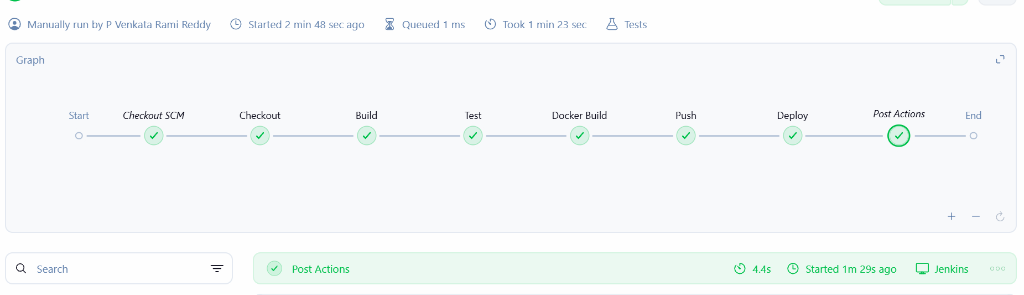
\includegraphics[width=0.98\textwidth]{screenshots/screenshot_a_jenkins.png}
    \caption{Green Jenkins declarative pipeline execution graph (all stages passing from Checkout through Deploy and Post Actions).}
    \label{fig:jenkins}
\end{figure}

\begin{figure}[htbp]
    \centering
    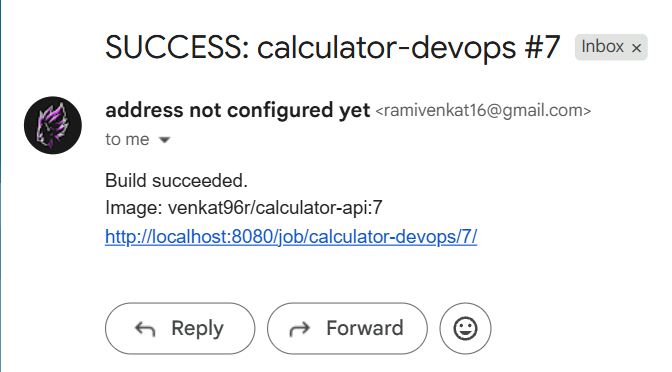
\includegraphics[width=0.80\textwidth]{screenshots/screenshot_b_email.png}
    \caption{Build status email notification received in Gmail inbox with build number (\#7), image tag, and build URL.}
    \label{fig:email}
\end{figure}

\newpage

\begin{figure}[htbp]
    \centering
    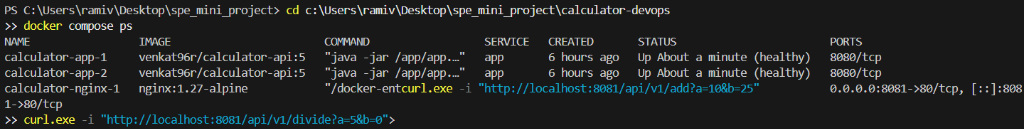
\includegraphics[width=0.98\textwidth]{screenshots/screenshot_c_docker_ps.png}
    \caption{\texttt{docker compose ps} output showing active Nginx reverse proxy on port 8081 and two healthy Spring Boot replicas.}
    \label{fig:dockerps}
\end{figure}

\vspace{0.8em}

\begin{figure}[htbp]
    \centering
    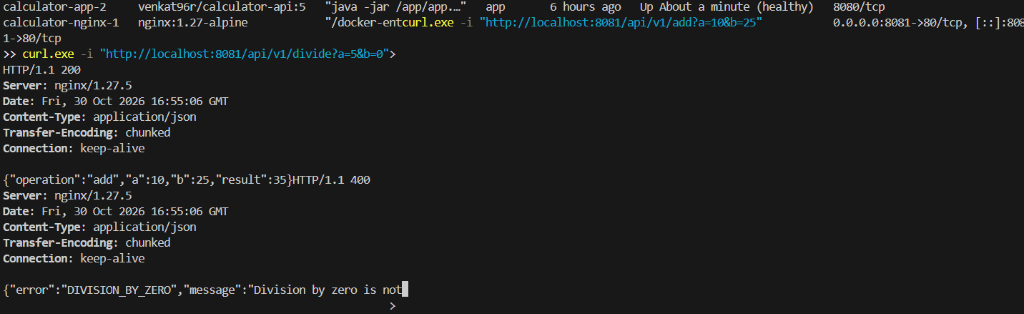
\includegraphics[width=0.98\textwidth]{screenshots/screenshot_d_sample_api.png}
    \caption{Sample API responses: successful addition calculation (HTTP 200 OK) and structured validation error for division by zero (HTTP 400 Bad Request).}
    \label{fig:api}
\end{figure}

\end{document}
